\chapter{Background}
\label{related-work}

\epigraph{Machines take me by surprise with great frequency.}{Alan Turing - 1950}

\section{Introduction}
This chapter aims to provide the context in which this work is written. By introducing the related scientific fields, this chapter sketches a broader context wherein this research exists. 

First, the field of information retrieval is introduced. Within the field of information retrieval, different approaches to \emph{retrieving information} have been used throughout the decades. These approaches will be introduced such that the reader understands what kind of techniques are used to retrieve information. The work described in this thesis would also be considered information retrieval research. 

Secondly, techniques from different research areas are also used for this research. Specifically, the research described in this thesis extensively uses techniques typically investigated by the \emph{data management} community. This field will also be introduced, where especially the techniques used for the research described in this work are highlighted. 

Then, the concept of \emph{graphs} will be explained. Graphs themselves are just mathematical structures that model the relations between objects. The objects are modeled as \emph{nodes} and relations between them as \emph{edges}. Many kinds of graphs exist; they are helpful for modeling problems that can be expressed formally through this framework. Different kinds of graphs will be explained, and examples of how to use them will be provided.

Finally, we will describe the idea of \emph{reproducible science}. In general, scientific work must be reproducible. In our research, we spend additional effort on reproducible science. What reproducibility exactly entails will be introduced.  

\section{Information Retrieval}
The research described in this thesis is \emph{information retrieval} research. Colloquially, one can refer to information retrieval as the science of everything relating to search engines. This field encompasses all aspects: from user experiences of search systems to storage algorithms and fast retrieval of the information items users search. \Citet{modern-information-retrieval} introduce information retrieval as the following:

\medskip
\textbf{Information retrieval (IR) deals with the representation, storage, organization of, and access to information items.}

\medskip
Following this description, an information retrieval system, i.e., a search engine, is a system that allows users to access information items that they are looking for. How this works internally is usually not interesting for the user, they want to find the information they need. Typically, and also in this thesis, the term \emph{document} refers to information items, even though the item the user seeks is not necessarily a literal document. 

Consider the following situation; someone wants to know whether it will rain in the coming 30 minutes. They might query a web search engine with the text \emph{weather}. In this case, the user does not care how the search engine works but only about the result. In order to satisfy the user's information need, the search engine needs to (1) present the correct weather forecast and (2) do this quickly. The user will be dissatisfied if the search engine presents the incorrect weather forecast or cannot do this in seconds.

In order to answer this inquiry for information correctly, the information retrieval system needs more context. It can only correctly know the weather if it is known where the user resides. When accessing search engines through a mobile device or computer, this information is sent along with the query as metadata. This way, the search engine can correctly answer even though the user did not explicitly give this information. 

When the user's location is known, the search engine needs to find a webpage that correctly provides the weather for that particular location. As there are billions of web pages in the search engine's index, correctly identifying which one contains information about the weather at that particular location and time and then retrieving it in seconds is the next challenge.

\subsection{Inverted Indexes}
Search engines must organize the data because it is infeasible to iterate over all web pages to check if the correct information is available. The most common data structure used in search engines is the inverted file.

Inverted indexes have been used for decades in the field of information retrieval. They are designed to access documents quickly. If a system cannot provide the data quick enough, the user is likely to switch to a different system. Documents are typically formed through words that form sentences, which form paragraphs, and, eventually, stories. When considering a document in its standard form, it is not trivial to determine efficiently whether it contains a specific word. When searching for something, it is paramount that the search engine knows what documents contain the keywords in the query. To efficiently access this data, instead of storing documents as is (a mapping from documents to words), search engines store the inverted information (a mapping from words to documents). To provide an example, consider the following three short documents:

\begin{itemize}
	\item[\textbf{1.}] Cats and dogs are animals.
	\item[\textbf{2.}] Cats are smart animals.
	\item[\textbf{3.}] Dogs are great at tricks. 
\end{itemize}
Then the inverted index looks something like this:

\medskip
\textbf{animal:} [1 2],
\textbf{cat:} [1 2], 
\textbf{dog:} [1 3],
\textbf{great:} 3,
\textbf{smart:} 2,
\textbf{trick:} 3
\medskip

\noindent A couple of interesting observations can be made here. Not all words appear in the inverted index. Typically words without ``meaning'', or so-called stop words, are removed. These words tend to contain no semantic information and can therefore be dropped. This process is called stopword removal or \emph{stopping}. Then, words are sometimes shortened to their \emph{stem}. Let us say we have a query only mentioning the word ``dog'', so not plural, then we still want to be able to find the documents that mention the plural form. This shortening to the word's stem is called \emph{stemming}. In this case, the words are ordered alphabetically. When the number of documents in a collection increases, the number of unique words also increases. By storing the words alphabetically, a computer can find the entries for that particular word more efficiently. 

When someone queries the search engine with the following query: ``dog tricks'', the search engine can directly find which documents contain these words using the inverted index. It can then automatically discard all documents that do not contain these words.
For the keywords, the search engine retrieves the lists associated with them. These lists are called \emph{posting lists} in information retrieval. Entries in such lists are referred to as \emph{postings}. In this case, the postings only contain the document identifiers as data. Generally, however, information like how often a word appears in a document or its location is also stored in the posting. In practice, posting lists are compressed, and instead of storing the direct identifiers, the gaps between them are stored such that the index becomes smaller. In literature, these gaps are referred to as delta gaps. 

In this case, the posting lists of the words ``dog'' and ``trick'' are retrieved: [1 3] and [3]. Then some scoring method can process these lists and assign a score to the documents present in these lists. As document 3 is the only document containing both words, it makes sense to consider this document the most relevant. However, assessing relevance ordering is more complicated when multiple documents contain both words with different frequencies. 
To create ranked lists of documents based on their estimated relevancy, different models for scoring documents have been proposed in the past. In the following sections, these models are presented.

\subsection{Ranking Models}

\subsubsection{Boolean Retrieval}\label{sec:boolean}
The Boolean retrieval model was used in the early days of information retrieval~\citep{boolean-1,boolean-2,rijsbergen79information}. Boolean retrieval can be formulated as the following; let, 

\begin{equation}
	T = \begin{Bmatrix}
		t_1, & t_2, & \ldots, & t_n
	\end{Bmatrix}
\end{equation}
be the set of all index terms that appear in the collection. Let,
\begin{equation}
	D = \begin{Bmatrix}
		d_1, & d_2, & \ldots, & d_m
	\end{Bmatrix}
\end{equation}
be the set of all documents, where every document is a subset of $T$. Specifically, the terms that appear in that document. Then a query can be any Boolean expression over $T$. All documents that adhere to the Boolean expression formed by the query are considered relevant. To give an example, consider the same three documents as before:

\begin{itemize}
	\item[\textbf{1.}] Cats and dogs are animals.
	\item[\textbf{2.}] Cats are smart animals.
	\item[\textbf{3.}] Dogs are great at tricks. 
\end{itemize}
Then, $D$ is formulated as $\left\{
\begin{smallmatrix}
	d_1, & d_2, & d_3 
\end{smallmatrix}
\right\}$ with,
\begin{align}
	d_1&: \begin{Bmatrix}
		\mathit{cat}, & \textit{dog}, & \textit{animal}
	\end{Bmatrix}\\
	d_2&: \begin{Bmatrix}
		\mathit{cat}, & \textit{smart}, & \textit{animal}
	\end{Bmatrix}\\
	d_3&: \begin{Bmatrix}
		\mathit{dog}, & \textit{great}, & \textit{trick}
	\end{Bmatrix}
\end{align}

One could be interested in finding all documents that mention dogs but not cats. Then we can formulate the following Boolean query:

\begin{equation}
	Q = \mathit{dog} \land \neg \mathit{cat}
\end{equation}

If we find all subsets that adhere to the individual terms in this conjunction, we get the following set expression:
\begin{equation}
	Q = \{d_1, d_3\} \cap \{d_3\} = \{d_3\}
\end{equation}
This shows that document $d_3$ is the only document that mentions dogs, but not cats. Although it is possible to express complicated expressions with Boolean logic, a document either satisfies the expression or does not. All documents that satisfy the expression are considered of equal importance; creating a ranking between them cannot be done with this approach alone. 

Using Boolean retrieval, there is no apparent difference between data retrieval and information retrieval; there is only one correct solution: all documents that satisfy the restrictions imposed by the query. 

\subsubsection{Vector Space Models}
In 1975, the vector space model was introduced by~\citet{VectorSpaceModel}. The idea behind the vector space model is to represent documents and queries as vectors. Consider a collection that has $t$ unique terms, then we can represent a document in the collection as a $t$ dimensional vector:
\begin{equation}
	D_j = \begin{pmatrix}
		w_0, \cdots, w_t
	\end{pmatrix}
\end{equation}
where $D_j$ is the $j$-th document in the collection, and $w_i$ represents the weight associated with the $i$-th term in the collection. These weights can be binary, or if one only wants to consider the importance of the term in the document, they can be the term frequency or any weight that considers the ``general'' term importance. 

Then if we have a query $q$, we can represent it in the same way:
\begin{equation}
	q = \begin{pmatrix}
		q_0, \cdots, q_t
	\end{pmatrix}
\end{equation}
where $q_i$ represents the weight of the $i$-th term in the collection. Most values in these vectors will be zero.

Now it is possible to calculate a similarity score between the query and every document. A widely used similarity metric is the cosine similarity between two vectors, which between a document $d$ and a query $q$ is defined as:

\begin{equation}
	\cos\left(d, q\right) = \frac{\textbf{d} \cdot \textbf{q}}{||\textbf{d}||\ ||\textbf{q}||}
\end{equation}

Calculating this for the documents in the collection gives an estimated value of relevance for all of them. Ordering them based on this estimated value then produces a ranked list where the highest is presumed to be the most interesting for the user. As mentioned before, the weights represented in the document vector do not necessarily have to be binary. \Citeauthor{VectorSpaceModel}~showed that the product of the term frequency with a general measure of term importance is highly effective. The measure they used for term importance was the inverse document frequency proposed by \citet{idf} three years earlier.

\subsubsection{Probabilistic Relevance Models}
\label{sec:probabilistic-relevance-models}
In 1976,~\citeauthor{RSJ} developed the probabilistic ranking framework. Within this framework, it is assumed that a document has a certain probability of being relevant given a query. Then, a search system that implements models within this framework ranks documents with the highest probability of being relevant the highest.

Within this framework, making an assumption of binary independence, which is nicely explained by~\citet{bm25-beyond}, the so-called Robertson-Sp{\"a}rck Jones weight can be derived. When assuming that no relevance labels are available, this leads to an approximation of the classical inverse document frequency.

By extending this function to include within-document term frequency information and document length normalization, the well-known BM25 function can be derived. \cref{ir-using-relational-databases} will focus on this model, and additional information explaining this model will be presented there.

\subsubsection{Language Models}
Later, language models were proposed~\citep{croft_lm, hiemstra_lm, zhai_lm}. The idea behind language models is that documents are considered samples of language, and queries are modelled as the result of a generative process from these samples. This process generates terms in the query by randomly selecting one of the words from that sample. Let the probability of a document $d$ generating a term $t_i$ be:

\begin{equation}
	P(t_i|d) = \frac{\mathit{tf}_{t_i,d}}{\sum_t^d tf(t, d)}
\end{equation}
with $\mathit{tf}_{t_i, d}$ being the term frequency of term $t_i$ in document $d$. 

Then, if we have a query $Q$, it is possible to calculate the likelihood that a document sample generated this query, as we know for every term in the query what the probability is that one of the document samples generates that term with Bayes rule: 

\begin{equation}
	P(d|Q) = \frac{P(d) \times \prod_{q \in Q} P(q | d)}{P(q)}
\end{equation}

Assuming an uniform relevance prior for the documents, and the fact  that $p(q)$ is constant for all documents we can determine the document with maximum likelihood through:  

\begin{equation}
	P(d|Q)  \propto \prod_{q \in Q} P(q | d)
\end{equation}

There are some issues when we take the document with the maximum likelihood. First, if a query contains multiple terms, a document can only get a non-zero likelihood of generating that query if all query terms exist in that document. If this is not the case, the probability of generating that term would be zero. As we take the product of the individual probabilities of the query terms, if one of them would be zero, the product would also be. The second issue is that there is no term-independent specificity weighting. Terms with a higher degree of specificity should increase the probability of relevance more than ``filler'' words. The previously described inverse document frequency took care of this in the vector space model.

\Citet{smoothing} show that a simple smoothing technique addresses both issues at once. Instead of only considering the samples formed by the documents, a collection-wide sample is being used, in a mixture model. This collection-wide sample generates terms according to the frequency in which the terms appear in the collection:
\begin{equation}
	P(t_i|C) = \frac{\mathit{df}(t_i)}{\sum_t^C \mathit{df}(t)}
\end{equation}
With $C$ being the collection, and $df(t_i)$ the document frequency of term $t_i$; i.e., the number of documents in the collection in which term $t_i$ appears. Then, the probability estimated by the document sample is interpolated by the probability based on the collection sample:
\begin{equation}
	P(d|Q) \propto \prod_{q \in Q} \omega \cdot P(q | d) + (1 - \omega) \cdot P(q | C) 
\end{equation}
with $\omega$ being the smoothing factor, i.e., how much is the collection sample weighted against the document sample?

This technique is also known as Jelinek-Mercer smoothing \cite{jelinek-mercer}. Smoothing the probability estimates like this, solves both problems: As the collection sample contains all terms, it is no longer possible for probabilities generated by a specific term to be zero, so the resulting product will not be zero either. Words with a higher specificity also get a boost; words with a high specificity have a low probability of being generated by the collection sample, meaning that it is more important for a document to contain that word to achieve a high probability of relevance. Words with a low specificity have a smaller effect; the probability of them being generated by the collection sample is already relatively high. 

\subsubsection{Learning-to-Rank}
With the increase in compute power, learning-to-rank became a popular approach to ranking. The methods described in the previous sections can all be considered unsupervised learning methods if we look at them from a machine learning perspective. Learning-to-rank models would be considered supervised or reinforcement learning methods from that perspective. The goal is to learn a model that, given a query, ranks documents relevant to that query higher than those not relevant to that query. In general, there are three ways to achieve this; for all these methods, relevance labels are assumed to be available from which the function can be learned. Learning-to-rank methods are usually categorized into the following three categories: 

\paragraph{Pointwise} Pointwise methods are most comparable to standard regression methods (e.g.\ linear regression). The idea is to learn a function that directly estimates a document's relevance label. Consider that we have $n$ query-document pairs for which relevance labels are available, with $m$ independent variables per pair. The relevance labels for these pairs can then be expressed as a vector $\mathbf{y}$, and the independent variables as a matrix $\mathbf{X}$:

\noindent\begin{minipage}[b]{.45\linewidth}
	\begin{align}
		\mathbf{y} = 
		\begin{bmatrix}
			y_1 \\
			\vdots \\
			y_n
		\end{bmatrix}
	\end{align}
\end{minipage}
\begin{minipage}[b]{.45\linewidth}
	\begin{align}
		\mathbf{X} = 
		\begin{bmatrix}
			x_{1,1} & \cdots & x_{1, m} \\
			\vdots &  \ddots & \vdots \\
			x_{n,1} & \cdots & x_{n, m} 
		\end{bmatrix}
	\end{align}
\end{minipage}


The goal would be to learn a function $\mathbf{\hat y} = f(\mathbf{X})$ such that some distance measure between $\mathcal{L}\left(\mathbf{\hat y}, \mathbf{y} \right)$ is minimized. Commonly used measures for this are mean square error or mean absolute error. The pointwise learning approach to ranking has some undesirable effects, however. Consider a situation where we have three documents; 
$\left[
\begin{smallmatrix}
	d_1, & d_2, & d_3
\end{smallmatrix}
\right]$, with relevance labels
$\left[
\begin{smallmatrix}
	1, & 0, & 0
\end{smallmatrix}
\right]$, i.e.\ document $d_1$ is relevant and the other documents are not. Then, two different ranking functions, $a$ and $b$, might produce the following relevance estimates: 
$a = \left[
\begin{smallmatrix}
	1, & 0.9, & 0.8
\end{smallmatrix}
\right]$ 
and
$b = \left[
\begin{smallmatrix}
	0, & 0.1, & 0.2
\end{smallmatrix}
\right]$, which results in the following respective rankings:
$\left[
\begin{smallmatrix}
	d_1, & d_2, & d_3
\end{smallmatrix}
\right]$ 
and 
$\left[
\begin{smallmatrix}
	d_3, & d_2, & d_1
\end{smallmatrix}
\right]$. 
The ranking produced by system $a$ is objectively better. It ranks the relevant document as the most relevant. System $b$, however, ranks the relevant document as the least relevant. If we evaluate the two systems with a loss function like mean absolute error however, system $b$ would seem the better one as the mean absolute error to
$\left[
\begin{smallmatrix}
	1, & 0, & 0
\end{smallmatrix}
\right]$
is smaller. 

\paragraph{Pairwise} Pairwise ranking tries to deal with this problem by not directly learning from the relevance labels but by looking at the relative preferences between pairs of documents. The idea behind this is that it does not matter what the actual ranking score value is, as long as it is higher for relevant documents than for non-relevant ones.  

Pairwise functions consider, given a query, two documents at a time. The function tries to determine which one of the two documents is more relevant than the other. If we consider the same set of relevance labels $\mathbf{y}$ and independent variables $\mathbf{X}$, then if we would take a pair of documents $x_k$ and $x_l$, with their corresponding relevance labels $y_k$ and $y_l$, assuming $y_k \neq y_l$, then we will learn the following function:
\begin{equation}
	f(x_k, x_l) = \begin{cases}
		0 & \text{if } y_k < y_l \\
		1 & \text{if } y_k > y_l
	\end{cases}
\end{equation}
This function can be learned by any binary classification method. After the method is learned, it can be used to determine an ordering of documents. 
Pairwise methods tend to be more expensive than pointwise methods, as the number of samples to train on for pointwise methods is $n$, with $n$ being the number of documents for which relevance assessments are available per query. For pairwise methods, every document with a label can be compared with every other document, creating $n^2$ training samples per query. 

A disadvantage of pairwise methods is that every pair is treated equally when training a model. There is no difference when comparing the two highest-ranked documents to comparing the two lowest-ranked documents, even though users typically care about the highest-ranked documents~\citep{pres-bias}. 

\paragraph{Listwise} Instead of looking at pairs of documents only, the listwise approach considers the whole ranking. This way, the top of the ranking can affect the function's learning more than the bottom of the ranking. Generally, when learning a listwise learning-to-rank method, the goal is to optimize some ranking metric quality directly. For example, LambdaMart~\cite{lambdamart} calculates what the differences on ranking metrics are by virtually swapping documents, these differences are used for determining gradients. (The gradients can not be calculated directly as the evaluation metric is not continuous with respect to the model parameters.) Examples of ranking metrics will be introduced in~\cref{sec:evaluation}.

\paragraph{Multistage Ranking}
\label{sec:multistage}
In many cases, applying inference to all documents in the collection is prohibitively costly. To reduce computational costs, multi-stage ranking is often used~\citep{multi-stage}.
A non-learning-to-rank approach is often used to create an initial ranking, under the assumption that the top-$k$ documents contain all relevant documents. The learned method only reorders the top-$k$ documents to present to the user. 

In these cases, it can make sense to rank the top-$k$ documents using an inverted index, while the reranking is done with another ranking approach.

\subsubsection{Vector Space Models revisited}
With the rise of large language models after the introduction of BERT by~\cite{BERT}, the vector space model has become more popular again due to what is called \emph{dense} retrieval.  

The basic idea is to estimate the relevance of a document $d$ for a query $q$ as follows:
\begin{equation}
	\text{rel}(q, d) = \omega\left(\phi\left(q\right),
	\psi\left(d\right)\right)
\end{equation}
Here, $\psi$ and $\phi$ are learned functions that use large language models to map the query and the document to vectors with relatively low dimensionality~\citep{seperation-logical-physical}.\footnote{$10^2$ - $10^3$ instead of the $10^8$ - $10^9$ parameters of the LLM's.} These functions map the query and the document to the same space. When documents are relevant to the query, the resulting vectors should be similar, while if the document is not relevant, they should be dissimilar, as measured through a similarity function $\omega$, often the dot-product or cosine similarity.

Finding the vectors closest to a query vector then corresponds directly to the nearest neighbor search problem. In the case of dense retrieval, dedicated dense retrieval systems (e.g.\ FAISS~\citep{faiss}) tend to be used instead of an inverted index. 

\subsection{Evaluation}
\label{sec:evaluation}
In the previous section, a variety of ranking approaches has been introduced. When comparing different ranking methods to each other, we need to be able to measure the quality of a result list for a given query. Many metrics have been introduced in the literature. Here, we focus on the most common evaluation metrics, including all the metrics used in this thesis. 

The metrics are $@k$ metrics, these only evaluate the documents ranked up to rank $k$, i.e., if $k=30$, we only consider the first $30$ documents produced by the system.

\subsubsection{Precision}
A straightforward approach to evaluating a ranking produced by a system is through precision. The precision metric counts the number of relevant documents found by the system, which is then divided by the total number of documents found by the system:
\begin{equation}
	\textit{P}@k = \frac{\sum_{i=1}^k\text{rel}\left(d_i\right)}{k}
\end{equation}
In this case, $\text{rel}(.)$ is a function that returns 1 if the document is relevant; otherwise, 0.
If $k=30$, then only the first $30$ documents are considered. If ten of these documents are relevant, then $P@30 = \frac{10}{30} = \frac{1}{3}$. Precision can, however, be somewhat limited in its use. In this example, the quality of the ranking might not seem good, as only a third of the produced documents are relevant. However, when only ten relevant documents are present in the collection, the $P@30$ found is the maximum attainable.  

\subsubsection{Recall}
Another approach to evaluate a ranking would be to measure how many relevant documents were retrieved compared to the total number of relevant documents in the collection. This measure is called recall: 
\begin{equation}
	\textit{R}@k = \frac{\sum_{i=1}^k\text{rel}\left(d_i\right)}{\sum_{i=1}^N\text{rel}\left(d_i\right)}
\end{equation}
Here $N$ is the number of documents in the collection. If, again, $k=30$ and we found $10$ relevant documents out of $15$ known relevant documents in the collection, then $R@30 = \frac{10}{15} = \frac{2}{3}$. The problem with recall is that it does not distinguish well between systems if only few relevant documents exist. Also, it is far from straightforward to determine the total number of relevant documents for an arbitrary query.

\subsubsection{Average Precision}
Consider the situation where three documents are retrieved, and two systems might produce rankings with the following relevance labels: $\left[
\begin{smallmatrix}
	1, & 0, & 0
\end{smallmatrix}
\right]$ and $\left[
\begin{smallmatrix}
	0, & 0, & 1
\end{smallmatrix}
\right]$.
Both rankings achieve the same $P@3$ and $R@3$ scores, and subsequently also the same $F_1@3$. The previously introduced metrics cannot distinguish between ranking quality in this situation. It is, however, clear that the order of documents in the first ranking should be preferred over the document-list in the second ranking. 
Instead of measuring the precision only at rank $k$, the average precision measure calculates it every time a relevant document is encountered. The sum of these values is divided by the number of relevant documents found up to $k$:
\begin{equation}
	\textit{AP}@k = \frac{1}{\sum_{i=1}^N\text{rel}\left(d_i\right)}\sum^k_{i=1} P\left(i\right) \cdot \text{rel}\left(d_i\right)
\end{equation}
Looking back at the two rankings, 
$\left[
\begin{smallmatrix}
	1, & 0, & 0
\end{smallmatrix}
\right]$ and $\left[
\begin{smallmatrix}
	0, & 0, & 1
\end{smallmatrix}
\right]$, the rankings produce an $\textit{AP}@3$ of $1$ and $\frac{1}{3}$, respectively.

\subsubsection{(Normalized) Discounted Cumulative Gain}
Discounted cumulative gain is an evaluation metric developed after the observation that users often only look at the highest-ranked documents and that documents might not have binary relevance labels (when we refer to their labels as graded relevance assessments)~\citep{ndcg}.
If a document is ranked at, say, rank 5, it might be possible that it is not considered by the user anymore, because they would rather reformulate the query. Plus, the metrics described before would rank the following two rankings to be of equal quality: 
$\left[
\begin{smallmatrix}
	2, & 1, & 0
\end{smallmatrix}
\right]$ and $\left[
\begin{smallmatrix}
	1, & 2, & 0
\end{smallmatrix}
\right]$
Discounted cumulative gain was developed with the intention that there should be a discounted gain every time a new relevant document is found, while non-binary relevance labels can be taken into account. This discount is applied by dividing by the logarithm of the rank plus one: 
\begin{equation}
	\textit{DCG}@k = \sum^k_{i=1} \frac{\text{rel}(d_i)}{\log_2(i+1)}
\end{equation}
In this case, $\text{rel}(\cdot)$ does not return a binary value but the actual relevance assessment label value.

A disadvantage of $\textit{DCG}$ is that the scores produced by this metric can vary greatly between rankings. If many highly relevant documents exist for a query, the values $\textit{DCG}$ takes can be much higher than if only one moderately relevant label is available. Normalized discounted cumulative gain takes care of this by dividing by the highest possible $\textit{DCG}$ that can be achieved. So normalized discounted cumulative gain is calculated by dividing the $\textit{DCG}$ of the ranking, by the $\textit{DCG}$ of the ideal ranking:  
\begin{equation}
	\textit{NDCG}@k = \frac{\textit{DCG}@k}{\textit{IDCG}@k} 
\end{equation}
with $\textit{IDCG}@k$ being the $\textit{DCG}@k$ for a perfect ranking. 

\subsubsection{Reciprocal Rank} 
The metrics described before score the whole ranking up to rank $k$. This might be unnecessary, for example, in a question answering scenario. If a document found is relevant, it may not matter anymore what the relevance assessment of the remaining documents. After all, the user would already have the answer, and likely stop looking for more information. The reciprocal rank therefore takes only the first found relevant document into account. Reciprocal rank~\citep{mrr} is the inverse of the index of the first found document:
\begin{equation}
	\textit{RR@k} = \frac{1}{\text{rank}(d)}
\end{equation}
where only the first $k$ documents are considered. Here, rank($d$) refers to the position of the first found relevant document. If the index of the first relevant is greater than $k$, the resulting score is $0$.

\subsection{Significance Testing}
Some of the measures described above can still be problematic when they are used to compare different ranking approaches. It is not always entirely clear how to do significance testing on some metrics. For example, \citet{fuhr-mrr} argues that in the case of reciprocal rank, the scores are not on an interval scale, but an ordinal one. It is not possible to calculate a mean score for an ordinal scale, which is however necessary for the most common tests for significance. \Citeauthor{fuhr-mrr} describes this, and other mistakes made when evaluating IR systems, plus how to avoid them. There are however some contrary views~\citep{on-fuhrs-guideline} that do not necessarily agree with these views. Specifically, \citeauthor{on-fuhrs-guideline} argues that are cases where ordinal is often averaged, and tested with parametric tests; for example in the case of multi-point scale ratings in user studies. To \citeauthor{on-fuhrs-guideline} it also not completely clear if Reciprocal Rank cannot be considered as a interval scale.

\section{Data Retrieval}
In the case of information retrieval, the concept of \emph{relevance} is critical. When someone issues a query, it does not necessarily have to be the case that words in the query must be present for the document to be relevant. Information retrieval has to deal with the uncertainty inherent to the information seeking process. Also, if only some relevant documents are found, this does not necessarily have to be a problem, as long as the information need of the user is satisfied. If we think about a search engine from a user's perspective, a document is only relevant if it contains the information they seek. In order to find this information, the user has to express their information need in a query, which the systems then have to interpret somehow in order to present the user (hopefully) the correct information. 
It might, however, be possible that two different users issue the same query, e.g., \emph{the weather}. Suppose one user is interested in today's weather, while the other is interested in tomorrow's weather. Different documents will be relevant for the user in these cases: relevancy is also tied to the user's expectations, that may not be known to the system.

In the field of \emph{data retrieval}, the notion of relevancy does not exist. When we speak about data retrieval, we are interested in retrieving all data that fulfills some \emph{predicate}. A predicate is a function that takes some input,\ i.e. the data, and it returns either true or false. In data retrieval we are interested in the data for which such a predicate resolves to true. It assumes that there is no ambiguity in the data and the request for data. An example query could be; to provide a list of all dog breeds. In this case, the system should return a list of all dog breeds known by the system. If it would accidentally forget to return one dog breed or includes an answer that is not correct, the system works incorrectly. 
The most commonly used data retrieval systems are relational database management systems (RDBMS) or relational databases. Relational databases represent tabular data as relations, a concept of from relational algebra; where a relation is defined as a set of tuples. In a relational database, a table corresponds to the relation, a row is one of the tuples, and a column can be considered an attribute in the tuple. Relational databases implement the operators as defined by relational algebra, which means users can select columns from a table (projection), filter rows that fulfill certain predicates (selection), and combine tables into new ones (join). There are differences between the theoretic framework of relational algebra and its wide-spread implementation in relational databases. For example, in practice, it is often possible to have duplicate rows in a relational database, which is inconsistent with a set. 

In the 1970s, relational databases have standardized on the structured query language (SQL).  
SQL is a declarative language; expressions specify which data needs to be retrieved, but not how. Depending on what a user expects from the program, choosing different database management systems for different applications makes sense. In the case of storing employee records for a company, it makes sense to store this data in a database suited for online \emph{transaction} processing (OLTP). Processing a transaction means that we update the data; e.g.\ adding new data to a table. When data analysis for scientific studies is important, storing data in a database system focused on online \emph{analytics} processing (OLAP) makes more sense. With analytics we mean queries that retrieve data as opposed to queries that update the data.  

\subsection{Physical vs. Logical models}
As SQL is a declarative language, data management systems' physical and logical models are strongly separated. Although many dialects of SQL exist, basic SQL queries are system agnostic and can run on different types of SQL engines. The logical model of data management systems are the SQL queries; what should be done. The physical model is how this should be done. Depending on which system is used, things like join ordering, how the data is processed, or how it is represented internally, can be very different. The logical model does not ``mind'' how the query is resolved, as long as it is done correctly. 

In the case of information retrieval, the physical and logical models are often more entangled. Model specification and query processing often co-exist. When this is the case, it can be harder to detect why systems differ when they implement the same models. \Cref{ir-using-relational-databases} will highlight this in more detail. 

\citet{seperation-logical-physical} discusses how information retrieval might benefit from separating physical and logical models in the context of dense retrieval models. \Cref{from-tables-to-graphs} will discuss his proposal in more detail.

\subsection{Columns vs. Rows}
Earlier database management systems were row oriented. Row-oriented means that when we look at how data is physically stored on the computer, all data within a tuple is represented near each other in memory. This orientation is especially well suited when a database needs to process many transactions. In the past, some IR systems have been built on top of such databases. However, these were much less efficient than when inverted indexes were used. Later, column-oriented databases were developed~\cite{column-oriented,monet}. These databases are more suited for analytical queries, at the cost of more expensive transaction processing. As these databases are designed for efficient and scalable analytics, they are also more suited for information retrieval systems. This practice is used throughout this thesis. 

\subsection{NoSQL and Graphs}
\label{sec:nosqlgraph}
In recent years there has been interest in database systems that approach data retrieval differently than traditional relational database systems~\citep{nosql}. These systems approach data retrieval without relying on the relational model. This could, for example, mean that joins are inefficient or not even possible to express within the system. This might seem limiting, but if certain operations are not supported, it might be possible to increase the efficiency of other operations. A very efficient key-value store like BigTable~\citep{bigtable} is a good example to illustrate this trade-off.

In particular, graph database (e.g.\ Neo4J\citep{neo4j}) systems are a type of NoSQL database management systems that have been of interest in the database community in the last few years. The concept of graphs is explained in \cref{sec:graphs}. The research presented in~\cref{from-tables-to-graphs} explores the possible benefits of considering these databases from an IR point of view.

\subsection{Embedded Databases}
Database management systems usually run on dedicated database servers. It is, however, also possible to use so-called embedded database systems. These systems do not require a dedicated database server, but work within the application process itself. An advantage of embedded databases is that they share memory space with the application process. This makes it possible to instantly move data from the database to a usable format for the application process. For information retrieval applications, this might be beneficial, especially in the case of multistage ranking approaches as described in ~\cref{sec:multistage}. However, embedded databases might not be the best solution in every case. When a dedicated database server is run, it is easier for multiple clients to read and write to the same database simultaneously. 

\subsection{Databases for Information Retrieval}
As databases are designed for the purpose of data retrieval, they are especially suited for information retrieval in the case of Boolean retrieval. However, it is harder to express the models that capture relevancy using a purely data retrieval approach.
When expressing models that represent uncertainty, i.e.\ model a likelihood measure of relevance, much data must be processed efficiently—inverted indexes are used to select critical data quickly. Older (row-based) database systems were not efficient enough to retrieve all necessary data to create rankings and model uncertainty simultaneously. After columnar databases became prominent, it was possible to express simple ranking models that consider uncertainty, with query plans that can be executed in a reasonably efficient manner. In this thesis, we will use, column oriented databases for information retrieval problems. Specifically, MonetDB~\citep{monet}, a non-embedded columnar database, is used for the work presented in \cref{ir-using-relational-databases}, and DuckDB~\citep{duckdb}, an embedded column oriented database, is used for the work presented in \cref{from-tables-to-graphs,ch:mmead}.

\section{Graphs}
\label{sec:graphs}
As mentioned in~\cref{sec:nosqlgraph}, in this thesis, we present work where approach information retrieval using graphs. In this section we describe what a graph is and which kinds of graphs exist. The graphs definitions follow the descriptions by \citet{big-graphs} and \citet{angles2018property}.

\paragraph{Basic Graphs}
A \emph{graph} is a structure consisting of a set of objects where pairs of these objects can be related. Typically, these objects are called nodes or vertices, and the relation between a pair of objects is referred to as an edge. So more formally, a graph $G$ is a pair of vertices $V$ and edges $E$;
\begin{equation}
	G = (V, E)
\end{equation}
where $V$ is the set of vertices in the graph, and $E$ a set of pairs (sets with two elements) of vertices:
\begin{equation}
	E = \left\{\left\{v_1, v_2\right\} | \left\{v_1, v_2\right\} \in V^2\right\}
	\label{undirected-edges}
\end{equation}
Graphs  can be depicted graphically illustrated as a set of circles, where every circle represents a vertex. If an edge exists between two vertices, a line is drawn between the two circles. \Cref{basic-graph}, for example illustrates a graph with $V = \left\{x_1, x_2, x_3\right\}$ and $E = \left\{\left\{x_1, x_2\right\}, \left\{x_2, x_3\right\}\right\}$. It does not necessarily have to be the case that every vertex is included in at least one edge.

\begin{figure}
	\centering
	\begin{subfigure}{.32\textwidth}
		\centering
		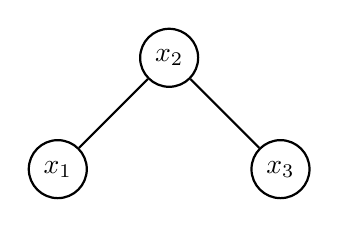
\begin{tikzpicture}[thick, node distance = {20mm}, main/.style = {draw, circle}] 
			\node[main] (1) {$x_1$}; 
			\node[main] (2) [above right of=1] {$x_2$};
			\node[main] (3) [below right of=2] {$x_3$};
			
			\draw (1) -- (2);
			\draw (2) -- (3);
		\end{tikzpicture}
		\caption{Basic Graph}
		\label{basic-graph}
	\end{subfigure}
	\hfill
	\begin{subfigure}{.32\textwidth}
		\centering
		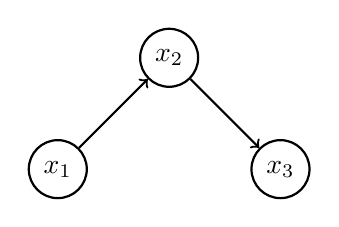
\begin{tikzpicture}[thick, node distance = {20mm}, main/.style = {draw, circle}] 
			\node[main] (1) {$x_1$}; 
			\node[main] (2) [above right of=1] {$x_2$};
			\node[main] (3) [below right of=2] {$x_3$};
			
			\draw[->] (1) -- (2);
			\draw[->] (2) -- (3);
		\end{tikzpicture}
		\caption{Directed Graph}
		\label{directed-graph}
	\end{subfigure}
	\hfill
	\begin{subfigure}{.32\textwidth}
		\centering
		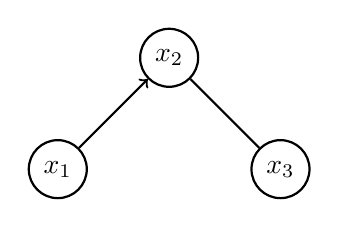
\begin{tikzpicture}[thick, node distance = {20mm}, main/.style = {draw, circle}] 
			\node[main] (1) {$x_1$}; 
			\node[main] (2) [above right of=1] {$x_2$};
			\node[main] (3) [below right of=2] {$x_3$};
			
			\draw[->] (1) -- (2);
			\draw (2) -- (3);
		\end{tikzpicture}
		\caption{Mixed Graph}
		\label{mixed-graph}
	\end{subfigure}
	
	\caption{Example of (\textbf{a}) a simple graph, (\textbf{b}) a directed graph, and (\textbf{c}) a mixed graph.}  
\end{figure}

A graph is called \emph{bi-partite} if it is possible to separate the set of vertices in two disjoint subsets,  such that  all edges only connect vertices from the two subsets with each other (there are no edges between vertices in the same subset). 

The graph's structure can be used to analyze how things relate. Considering geographical maps, we can model countries as vertices and create an edge between two countries if they are neighboring. Then, we can use the graph structure to analyze the possible paths from one country to another where only the fewest possible other countries are crossed, on a smaller scale this is useful for navigation systems. For many use cases, however, it is helpful to let graphs have less restrictive rules on how it might be formed.

\paragraph{Directed Edges} The most basic extension of graphs is that they are allowed directed edges. This means an edge can exist from one node to another, but this connection does not  automatically also exist in the opposite direction. In the case of countries and their neighbors, this does not make sense; if one country borders another, the opposite is also true. However, on the internet, one website might contain a hyperlink to another, while the opposite does not have to be the case. We need directed graphs to properly model the situation. Again, we can use this model to see how many paths exist from one website to another, with the restriction of visiting two other websites. In this case, $E$ is a set of ordered pairs of vertexes: 
\begin{equation}
	E = \left\{\left(v_1, v_2\right) | \left(v_1, v_2\right) \in V^2\right\}
	\label{directed-edges}
\end{equation}
\Cref{directed-graph} shows an illustration of the following directed graph:
$V = \left\{x_1, x_2, x_3\right\}$ and $E = \left\{\left(x_1, x_2\right), \left(x_2, x_3\right)\right\}$

\paragraph{Mixed Graphs}
Mixed graphs are graphs that accept both undirected and directed edges. In that case, a graph is defined with two sets of edges, where one set describes the undirected edges and the other the directed edges:
\begin{equation}
	G = \left\{V, E_1, E_2\right\}
\end{equation}
with $E_1$ and $E_2$ being defined as edges as presented in \cref{undirected-edges,directed-edges} respectively. \cref{mixed-graph} shows the illustration of a mixed graph:
$V = \left\{x_1, x_2, x_3\right\}$, $E_1 = \left\{\left\{x_1, x_2\right\}\right\}$, and $E_2 = \left\{\left(x_2, x_3\right)\right\}$.
Mixed graphs are sometimes used in applications where the direction of an edge is not known but it is clear that a relation exists. Types of these graphs appear, for example, in causality research. 

\subsection{Labeled Graphs} 
None of the types of graphs we described so far contain data themselves; we can only reason about the structure of the graphs. Even though this already has many practical applications, graphs are more useful for the applications we are interested in when they are allowed to contain data. There are two ways to add data to graphs; it is possible to add data to the vertices or the edges.

\begin{figure}
	\centering
	\begin{subfigure}{.49\textwidth}
		\centering
		\begin{tikzpicture}[thick, node distance = {20mm}, main/.style = {draw, ellipse}] 
			\node[main] (1) {$x_1 : 2$}; 
			\node[main] (2) [above right of=1] {$x_2: 2$};
			\node[main] (3) [below right of=2] {$x_3: 2$};
			\node[main] (4) [above right of=3] {$x_4: 1$};
			
			\draw[->] (1) -- (2);
			\draw[->] (2) -- (3);
			\draw[->] (3) -- (1);
			\draw[->] (4) -- (3);
		\end{tikzpicture}
		\caption{Data Graph}
		\label{data-graph}
	\end{subfigure}
	\hfill
	\begin{subfigure}{.49\textwidth}
		\centering
		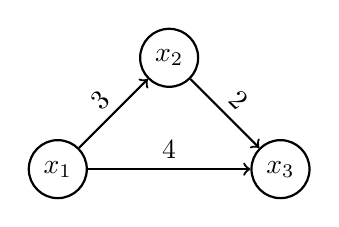
\begin{tikzpicture}[thick, node distance = {20mm}, main/.style = {draw, circle}] 
			\node[main] (1) {$x_1$}; 
			\node[main] (2) [above right of=1] {$x_2$};
			\node[main] (3) [below right of=2] {$x_3$};
			
			\draw[->] (1) --node[left, sloped, above]{3} (2);
			\draw[->] (2) --node[right, sloped, above]{2} (3);
			\draw[->] (1) --node[right, sloped, above]{4} (3);
		\end{tikzpicture}
		\caption{Weighted Graph}
		\label{weighted-graph}
	\end{subfigure} 
	\caption{Example of (\textbf{a}) a data graph, and (\textbf{b}) a weighted graph.}  
\end{figure}

\paragraph{Data Graph}
A data graph is a type of graph where vertices have data. \Cref{data-graph} shows an example of a (directed) graph where every vertex is labeled with a number. These graphs are, for example, used in the PageRank algorithm~\citep{pagerank}. In this algorithm, every vertex represents a webpage, and a directed edge exists between a node $a$ to $b$ if a link on website $a$ points to website $b$. Then by randomly walking over this graph or visiting a new website randomly, it is possible to count how often a node has been visited. The number of visits corresponds to the PageRank score. Normalized PageRank scores correspond to the probabilities found in a Markov process in equilibrium.  

\paragraph{Weighted Graph}
A weighted graph is a type of graph where edges contain data. \Cref{weighted-graph} shows an example of a (directed) graph where every edge is labeled with a number. For example, these kinds of graphs are used to calculate the shortest distance between nodes. They are, for example, useful for navigation systems. There are two possible paths if we need to travel from location $x_1$ to location $x_3$. The path from $x_1$ directly to $x_3$ is shorter than going from $x_1$ to $x_3$ via $x_2$. When graphs are larger, algorithms like Dijkstra's algorithm can efficiently find the shortest path over weighted graphs.

\paragraph{Pregel/Giraph Graph}
An obvious extension of the data graph is, of course, adding data to both the vertices and edges. In this context, we refer to them as Pregel/Giraph graphs~\citep{pregel,giraph}, as these systems are widely used implementations of these graphs. Some algorithms need graphs to have both edge and vertex data. An example is the node2vec algorithm, which generates vector representations of the vertices of the graph. These graphs are used for various machine learning applications. 

Formally the data on the graph can be expressed by a labeling function:
\begin{equation}
	\rho : \left(V \cup E\right) \rightarrow w\text{ | }w \in \mathbb{R}^+
\end{equation}
In this case, we assume that the data are positive numbers, as often it is a constraint imposed by algorithms. There are however no theoretical restrictions from graph theory that impose this constraint.
The data graph and weighted graph can be expressed with the same labeling function, with just the vertices or the edges as input for the labeling function. 

\subsection{RDF graphs}

\begin{figure}
	\centering
	\begin{tikzpicture}[thick, node distance = {45mm}, main/.style = {draw, ellipse}] 
		\node[main] (1) {Chris}; 
		\node[main] (2) [right of=1] {Arjen};
		\node[main] (3) [left of=1] {Kamphuis};
		
		\draw[->] (1) edge[] node[left, below] {knows} (2);
		\draw[->] (1) edge[bend right=45] node[left, below] {learnsFrom} (2);
		\draw[->] (1) edge[] node[left, below] {lastName} (3);
	\end{tikzpicture}
	\caption{Example of a W3C RDF graph.} 
	\label{rdf-graph} 
\end{figure}

Research Description Framework (RDF) graphs are directed graphs where edges have labels and where multiple edges may exist between a pair of nodes. Graphs that allow multiple edges between a pair of nodes are also called \emph{multi-graphs}.
They are a standard by the World Wide Web Consortium (W3C). The idea behind RDF graphs is that they can be resolved by a collection of so-called triples. These triples contain a \emph{subject}, \emph{predicate}, and \emph{object}. The predicate describes the relation (edge) between the subject (node) and the object (node); a collection of triples forms a graph. RDF graphs are widely used to represent knowledge graphs. These are widely used to store information about named \emph{entities}; things in the real world like persons, locations, or organizations. As a rule of thumb, you could say that everything that could have a Wikipedia entry can be considered a named entity. Knowledge graphs have many applications in information retrieval. It is, for example, possible to generate entity cards~\citep{entity-cards} on top of search engine result pages using knowledge graphs. \Cref{rdf-graph} shows an example of a small RDF graph. 

\subsection{Property Graphs}
\begin{figure}
	\centering
	\begin{tikzpicture}[thick, node distance = {65mm}, main/.style = {draw, ellipse}] 
		\node[main, align=center] (1) {\underline{Chris} \\ \textit{lastName:} Kamphuis \\ \textit{born:} 1993 }; 
		\node[main] (2) [right of=1] {\underline{Arjen}};
		
		\draw[->] (1) edge[align=center, bend right=45] node[left, below] {knows \\ \textit{since:} 2014} (2);
		\draw[->] (1) edge[] node[left, below] {learnsFrom} (2);
	\end{tikzpicture}
	\caption{Example of a Property Graph.} 
	\label{property-graph} 
\end{figure}

The final type of graph we discuss is the property graph. Property graphs allow everything we described before, while vertices can also have labels, and vertices and edges can have property-value pairs (multiple values per property are even allowed). A property-value represents some named data for either a vertex or edge. For example, if a node represents a person, the person's age can be a property of the node. Depending on the type of property graph, the graph might also contain multiple vertex or edge labels. \cref{property-graph} shows an example of a property graph. The node with label \emph{Chris} has last name and birth year properties. The edge with label \emph{knows} from the node \emph{Chris} to the node \emph{Arjen} has a timestamp as a property. Property graphs have high expressive power, and have become the preferred data model for graph databases. 

Formally, to complement our previous definitions of vertices and edges, we assume the existence of three infinite sets; $L$, $P$, and $A$. $L$ is an infinite set containing vertex/edge labels, $P$ is an infinite set containing property names, and $A$ is an infinite set of atomic values. Using these sets we can define the following two functions that assign labels, and property-value pairs:
\begin{equation}
	\lambda : \left(V \cup E\right) \rightarrow l \text{ | } l \subset L
\end{equation}
\begin{equation}
	\sigma : \left(V \cup E\right) \times P \rightarrow a \text{ | } a \subset A
\end{equation}

In \cref{from-tables-to-graphs}, we built on this representation to explore graph databases for IR. 

\section{Reproducible Science}
In order to establish experimental results in science, it is essential that they can independently be verified. Many fields have had problems where the reproducibility of scientific studies fell short. In psychology, a large reproducibility study was carried out~\citep{psychology-reproduciblity}, based on a selection of 100 studies published in 2008. The goal was to reproduce the findings of all these studies, to determinethe state of reproducibility of the field. Of the original 100 studies, 97 presented significant results. However, when trying to reproduce these results, only 35 out of 97 of these studies succeeded to reproduce significant results. 

It is unclear why that many scientific studies were not reproducible. Nevertheless, many type II errors happened; failure to reject the null hypothesis while it is false. Scientific misconduct could explain some of these results, but it is unlikely that this is happening at such a large scale. All studies this project tried to reproduce were published in just three journals. These journals were peer-reviewed; only the scientific studies the reviewers thought were good enough were published. This process, of course, introduces a selection bias. Studies that show more impactful results have a higher probability of being published. This bias favors papers with type II errors, even when the scientific conduct was proper. 

When a scientific study is published, people might interpret its results as fact. However, one should consider experimental results only as evidence of how the world might work. Then, whenever the results are reproduced, more evidence is gathered to support the findings. By reproducing science, our understanding of the world becomes more precise, and eventually, we can assume with high certainty a hypothesis to be true. 

In the field of information retrieval, reproducibility has also been a topic of interest. Reproducibility is discussed several times in the dissertation, and only some observations on the topic of reproducibility in our field are highlighted here. Before introducing these observations, it is important to clearly define what is meant by reproducibility. Within the Association for Computing Machinery (ACM), a distinction has been made between the concepts of repeatability, replicability, and reproducibility\footnote{\url{https://www.acm.org/publications/policies/artifact-review-badging}, last accessed - August 25th 2025}: 
\begin{itemize}
	\item \emph{Repeatability} is verification of results produced by the \underline{same} research group, using the \underline{same} resources. Confirming that when one reruns their experiments, the same results are produced. This might seem trivial, but when software is updated to some newer version, the results that the software produces could differ slightly. 
	\item \emph{Replicability} is the verification of results produced by a \underline{different} research group, but using the \underline{same} resources. This could, for example, be done by running the publicly available code for a research project and verifying its results. This is more tricky than it might look. Often, for example in scientific papers, the exact parameter settings of the software might be left out, making it hard to verify results correctly. 
	\item \emph{Reproducibility} is the verification of results produced by a \underline{different} research group that uses its own (\underline{different}) resources. Typically, in a reproduction study, the scientific study is done from scratch using the instructions presented in a paper. As many details might be left out, it is even harder to reproduce results exactly. However, if a reproduction study can confirm the results of previous work, this is a strong indication of the correctness of the results presented in that work.
\end{itemize}

In \cref{ir-using-relational-databases}, we present empirical results about the BM25 algorithm. Many systems implement this algorithm, while the reported effectiveness results as measured through established metrics (a subset of metrics described in \cref{sec:evaluation}) vary substantially. How this can happen will be discussed. BM25, however, is a ranking method often used as a baseline method. When comparing newer algorithms to BM25, it makes quite a difference if its implementation reports a relatively low score, or a high one. 

\Citet{Armstrong-dontaddup} showed that many improvements in ranking algorithms presented throughout the years did not add up. Significant improvements were presented in many cases, where these were compared against weak baselines. Also, there was no upward trend of retrieval effectiveness, which would be expected if we find repeated improvements. More recently, \citet{weak-baselines} showed new methods are still being compared against implementations of BM25 that have non-optimal hyperparameter settings. This leads to methods that are less effective than presented. 

For this thesis, all software and data produced is publicly available and released on Zenodo\footnote{\url{https://zenodo.org}, last accessed - November 13th 2024} in order to facilitate reproducible science, following the guidelines of the research data management policy of the Institute for Computing and Information Science of the Radboud University\footnote{\url{https://www.ru.nl/rdm/}, last accessed - November 13th 2024 }. Additionally, in some chapters, the importance of reproducibility will be highlighted and discussed in more detail.  